% Created 2018-12-12 Wed 13:44
% Intended LaTeX compiler: pdflatex
\documentclass[11pt]{article}
\usepackage[utf8]{inputenc}
\usepackage[T1]{fontenc}
\usepackage{graphicx}
\usepackage{grffile}
\usepackage{longtable}
\usepackage{wrapfig}
\usepackage{rotating}
\usepackage[normalem]{ulem}
\usepackage{amsmath}
\usepackage{textcomp}
\usepackage{amssymb}
\usepackage{capt-of}
\usepackage{hyperref}
\usepackage{minted}
\usepackage[1.0in]{geometry}
\author{Mijeong Ban}
\date{\today}
\title{}
\hypersetup{
 pdfauthor={Mijeong Ban},
 pdftitle={},
 pdfkeywords={},
 pdfsubject={},
 pdfcreator={Emacs 26.1 (Org mode 9.1.9)}, 
 pdflang={English}}
\begin{document}


\section*{Part One. Statistical Report}
\label{sec:org1b0c1d5}

\section*{Part Two. Textbook Exercises}
\label{sec:org0bff31a}
\subsection*{11.42 Relationships among PCB congeners}
\label{sec:orge02c8ac}
Consider the following variables: PCB(the total amount of PCB) and four congeners: PCB52, PCB118, PCB138, and PCB180.
\subsubsection*{(a) Using numerical and graphical summaries, describe the distribution of each of these variables.}
\label{sec:org1fbb4b6}
\begin{table}[htbp]
\caption{Numerical Summaries}
\centering
\begin{tabular}{lrrrrrr}
Variable & Min & 1st Qu. & Median & Mean & 3rd Qu. & Max\\
\hline
PCB & 6.10 & 30.18 & 47.96 & 68.47 & 91.63 & 318.70\\
PCB52 & 0.020 & 0.228 & 0.477 & 0.958 & 0.892 & 9.060\\
PCB118 & 0.236 & 1.490 & 2.420 & 3.256 & 3.890 & 18.900\\
PCB138 & 0.640 & 3.180 & 4.920 & 6.827 & 8.650 & 32.300\\
PCB180 & 0.395 & 1.240 & 2.690 & 4.158 & 4.490 & 31.500\\
\end{tabular}
\end{table}

\begin{figure}[htbp]
\centering
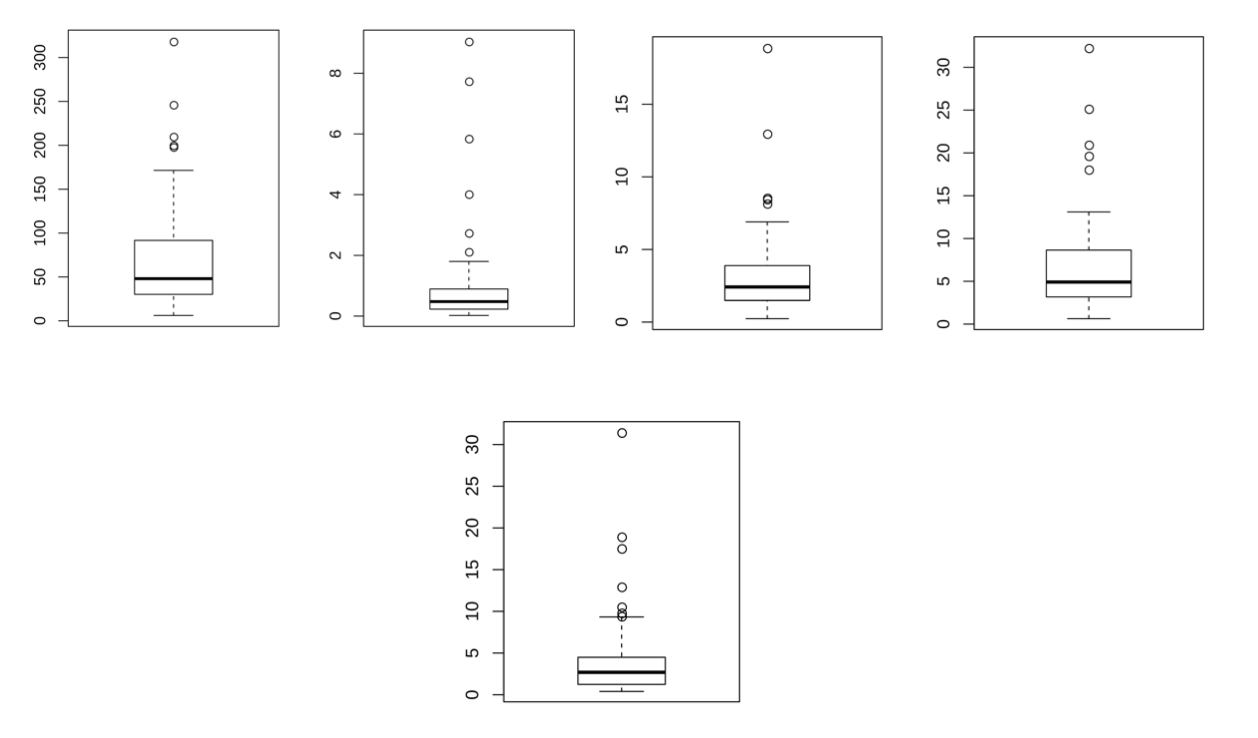
\includegraphics[width=.9\linewidth]{./graphs/image1.png}
\caption{Boxplots of PCB, PBC52, PCB118, PCB138 and PCB180}
\end{figure}
Figure 1 shows that the distribution of PCB and PCB180 is right skewed with about six outliers for both, while all the distribution of others are right skewed with about five outliers.  

\subsubsection*{(b) Using numerical and graphical summaries, describe the relationship between each pair of variables.}
\label{sec:org3aa9e19}
\begin{table}[htbp]
\caption{Correlations}
\centering
\begin{tabular}{llr}
Variable 1 & Variable 2 & Correlation\\
\hline
PCB & PCB52 & 0.5963572\\
PCB & PCB118 & 0.843298\\
PCB & PCB138 & 0.9288353\\
PCB & PCB180 & 0.8008549\\
PCB52 & PCB118 & 0.6849073\\
PCB52 & PCB138 & 0.3008983\\
PCB52 & PCB180 & 0.08692971\\
PCB118 & PCB138 & 0.7293792\\
PCB118 & PCB180 & 0.4374443\\
PCB138 & PCB180 & 0.8823022\\
\end{tabular}
\end{table}

\begin{center}
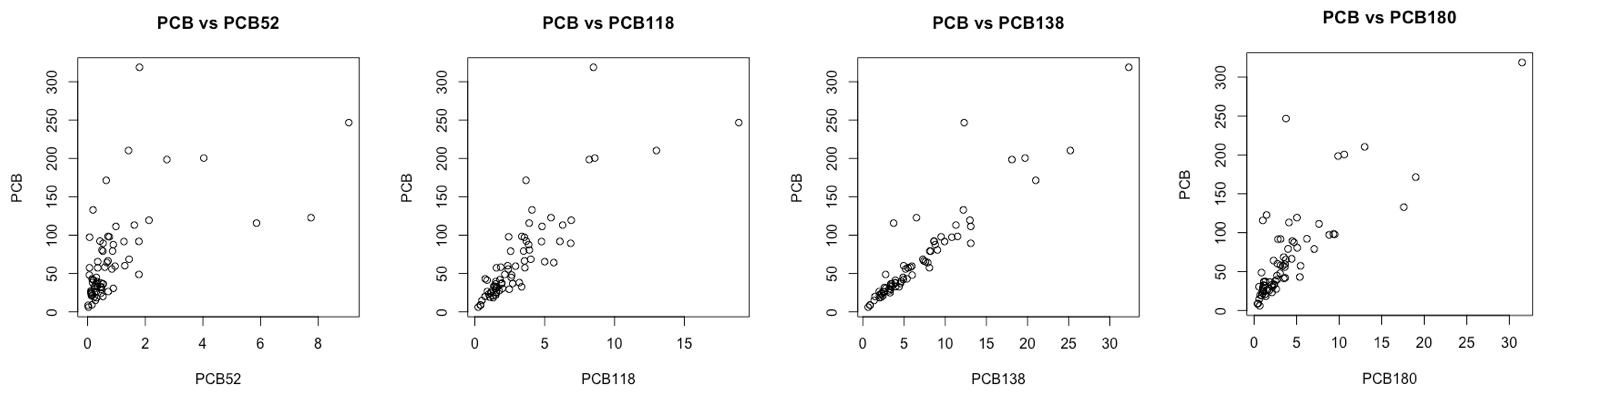
\includegraphics[width=.9\linewidth]{./graphs/image2.png}
\end{center}
\begin{center}
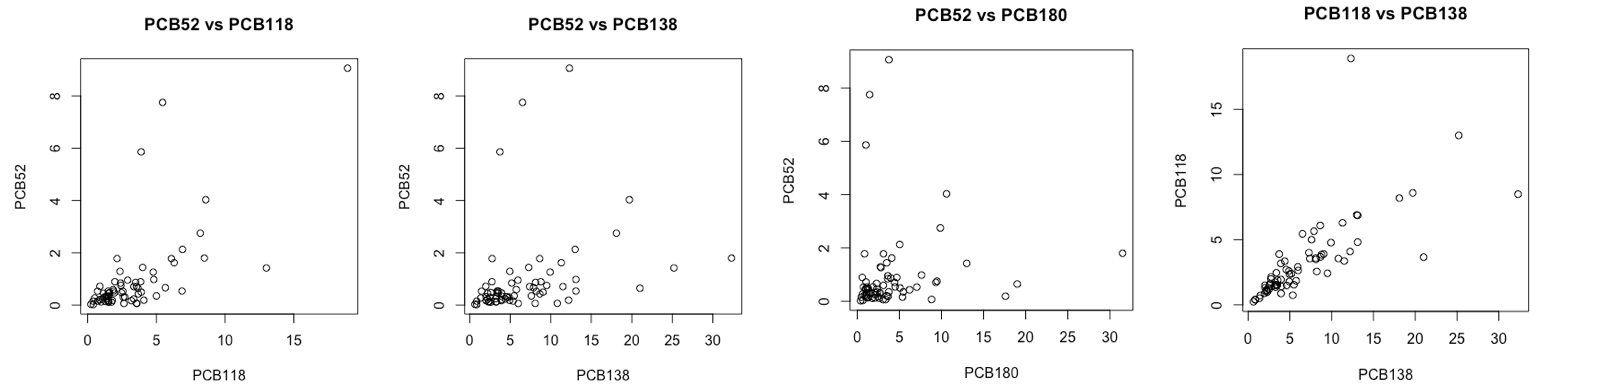
\includegraphics[width=.9\linewidth]{./graphs/image3.png}
\end{center}
\begin{center}
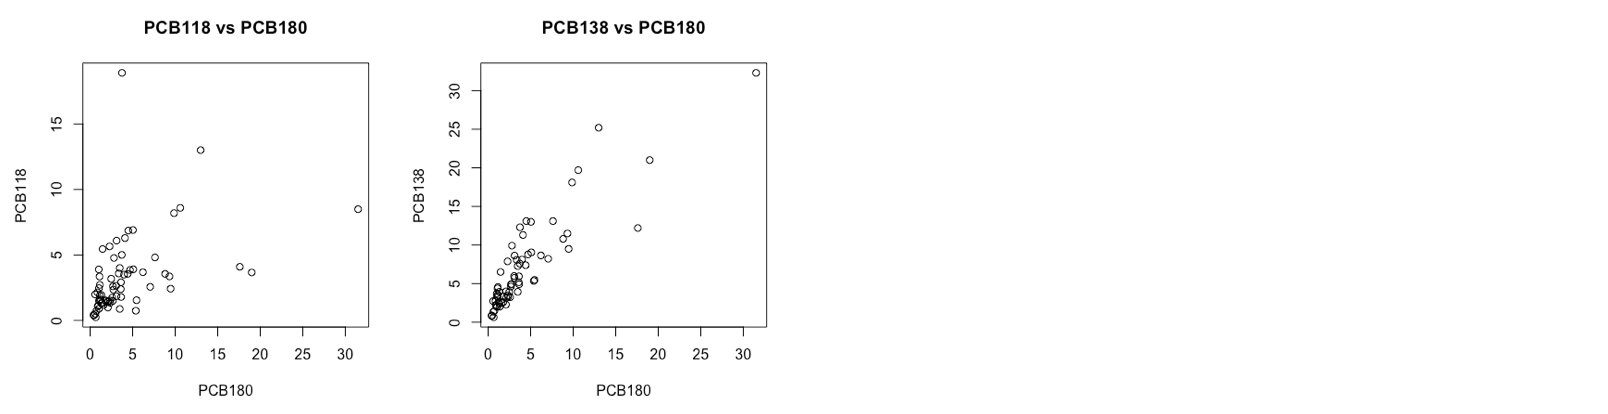
\includegraphics[width=.9\linewidth]{./graphs/image4.png}
\end{center}

\subsection*{11.43 Predictiong the total amount of PCB}
\label{sec:org1b4f413}
Use the four congeners PCB52, PCB118, PCB138, and PCB180 in a multiple regression to predict PCB. 
\subsubsection*{(a) Write the statistical model for this analysis. Include all assumptions.}
\label{sec:orgca5dcdc}
The multiple linear regression model for the data with 69 observations:

y\(_{\text{i}}\) = \(\beta_{\text{0}}\) + \(\beta_{\text{1}}\)x\(_{\text{i1}}\) + \(\beta_{\text{2}}\)x\(_{\text{i2}}\) + \(\beta_{\text{3}}\)x\(_{\text{i3}}\) + \(\beta_{\text{4}}\)x\(_{\text{i4}}\) + i \emph{for} \emph{i = 1, 2, \ldots{} , 69}

We assume that the residuals are independent and are normally distributed. 
\subsubsection*{(b) Run the regression and summarize the results.}
\label{sec:org1d30215}
Multiple regression analyses were conducted to examine the relationship between PCB and four congeners. Running the multiple regression model in R with the four congeners produced the following:
\begin{verbatim}

subdf <- subset(df, select = c("pcb", "pcb52", "pcb118", "pcb138", "pcb180"))
> lm1 = lm(pcb~pcb52 + pcb118 + pcb138 + pcb180, data=subdf)
> coef(lm1)
(Intercept)       pcb52      pcb118      pcb138      pcb180 
  0.9369203  11.8726953   3.7610694   3.8842264   4.1823010 
> summary(lm1)

Call:
lm(formula = pcb ~ pcb52 + pcb118 + pcb138 + pcb180, data = subdf)

Residuals:
     Min       1Q   Median       3Q      Max 
-22.0864  -2.4554   0.0278   2.7726  22.5487 

Coefficients:
            Estimate Std. Error t value Pr(>|t|)    
(Intercept)   0.9369     1.2293   0.762    0.449    
pcb52        11.8727     0.7290  16.287  < 2e-16 ***
pcb118        3.7611     0.6424   5.855 1.79e-07 ***
pcb138        3.8842     0.4978   7.803 7.19e-11 ***
pcb180        4.1823     0.4318   9.687 3.64e-14 ***
---
Signif. codes:  0 ‘***’ 0.001 ‘**’ 0.01 ‘*’ 0.05 ‘.’ 0.1 ‘ ’ 1

Residual standard error: 6.382 on 64 degrees of freedom
Multiple R-squared:  0.9891,	Adjusted R-squared:  0.9885 
F-statistic:  1456 on 4 and 64 DF,  p-value: < 2.2e-16

> anova(lm1)
Analysis of Variance Table

Response: pcb
          Df Sum Sq Mean Sq  F value    Pr(>F)    
pcb52      1  85302   85302 2094.273 < 2.2e-16 ***
pcb118     1  85429   85429 2097.405 < 2.2e-16 ***
pcb138     1  62693   62693 1539.202 < 2.2e-16 ***
pcb180     1   3822    3822   93.834  3.64e-14 ***
Residuals 64   2607      41                       
---
Signif. codes:  0 ‘***’ 0.001 ‘**’ 0.01 ‘*’ 0.05 ‘.’ 0.1 ‘ ’ 1
\end{verbatim}
\begin{itemize}
\item We gathered the following from the results of the regression:
\label{sec:orgf111c41}
\begin{itemize}
\item The multiple R\(^{\text{2}}\) = 0.989
\item The residual SE = 6.249
\end{itemize}
\end{itemize}

\item Test 1
\label{sec:org11293af}

H\(_{\text{0}}\) : \(\beta_{\text{0}}\) = \(\beta_{\text{1}}\) = \(\beta_{\text{2}}\) = \(\beta_{\text{3}}\) = \(\beta_{\text{4}}\) = 0

H\(_{\text{1}}\) : \(\beta_{\text{0}}\) \(\neq\) 0 \(\vee\) \(\beta_{\text{1}}\) \(\neq\) 0 \(\vee\) \(\beta_{\text{2}}\) \(\neq\) 0 \(\vee\) \(\beta_{\text{3}}\) \(\neq\) 0 \(\vee\) \(\beta_{\text{4}}\) \(\neq\) 0

Since there is at least one \(\beta_{\text{n}}\) \(\neq\) 0, we reject H\(_{\text{0}}\) 

\item Test 2
\label{sec:org0b2b635}

H\(_{\text{0}}\) = \(\beta_{\text{j}}\) = 0, \emph{j = 0, 1, 2, 3}

H\(_{\text{1}}\) = \(\beta_{\text{j}}\) \(\neq\) 0

All regression coefficients are significantly different from 0 with the except of 0.94. We found that R\(^{\text{2}}\) = 0.989, meaning that 98.9\% of variation in PCB is from PCB52, PCB118, PCB138 and PCB180.
\end{itemize}

\subsubsection*{(c) Examine the residuals. Do they appear to be approximately Normal? When you plot them versus each of the explanatory variables, are any patterns evident?}
\label{sec:org403a548}
\begin{center}
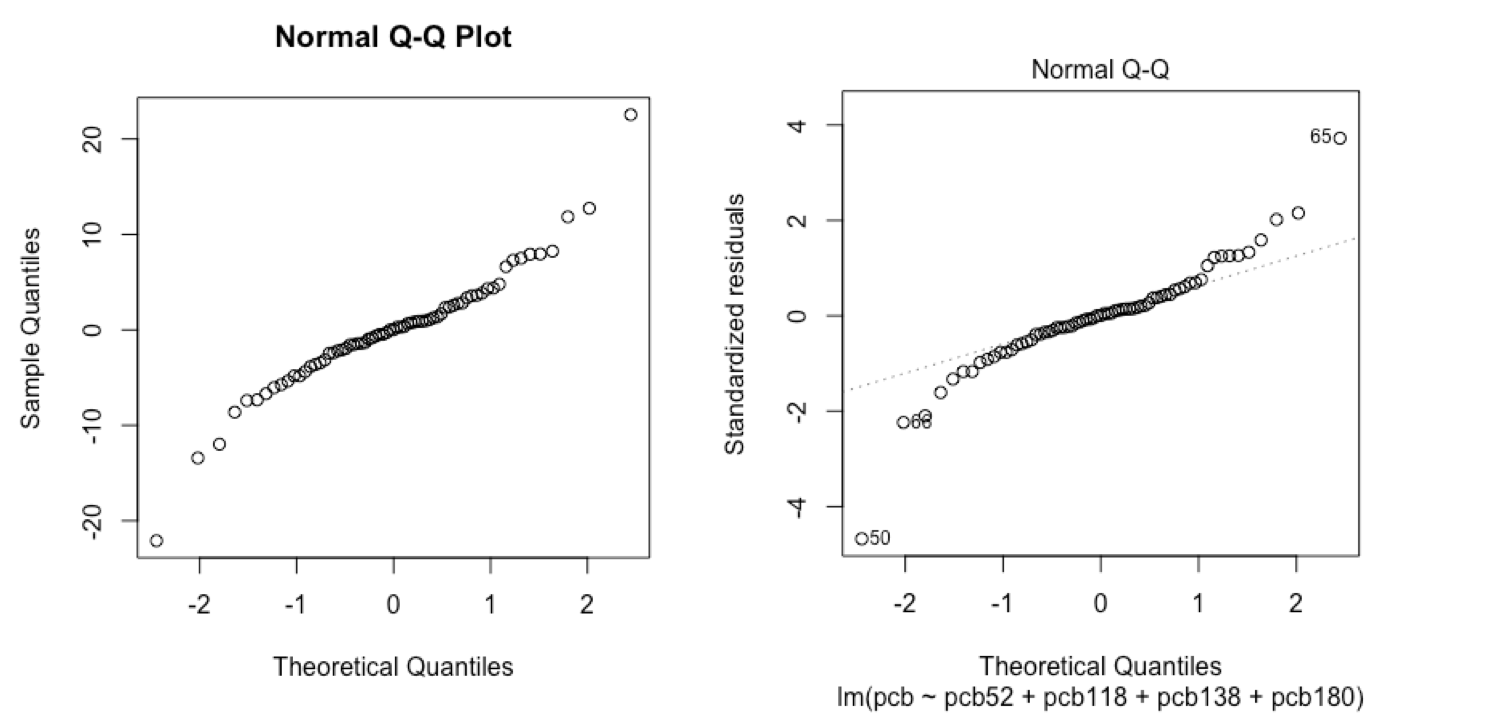
\includegraphics[width=.9\linewidth]{./graphs/image5.png}
\end{center}
According to the graphs, the residuals shows two clear outliers and shows that the residuals are approximately normal. Rhere are no other patterns in the explanatory variables of note. 

\subsection*{11.44 Adjusting the analysis for potential outliers.}
\label{sec:org65569ca}
The examination of the residuals in part (c) of the previous exercise suggests that there may be two outliers, one with a high residual and one with a low residual. 
\subsubsection*{(a) Because of safety issues, we are more concerned about underestimating PCB in a specimen than about overestimating. Give the specimen number for each of the two suspected outliers. Which one corresponds to an overestimate of PCB?}
\label{sec:org498242a}
\begin{center}
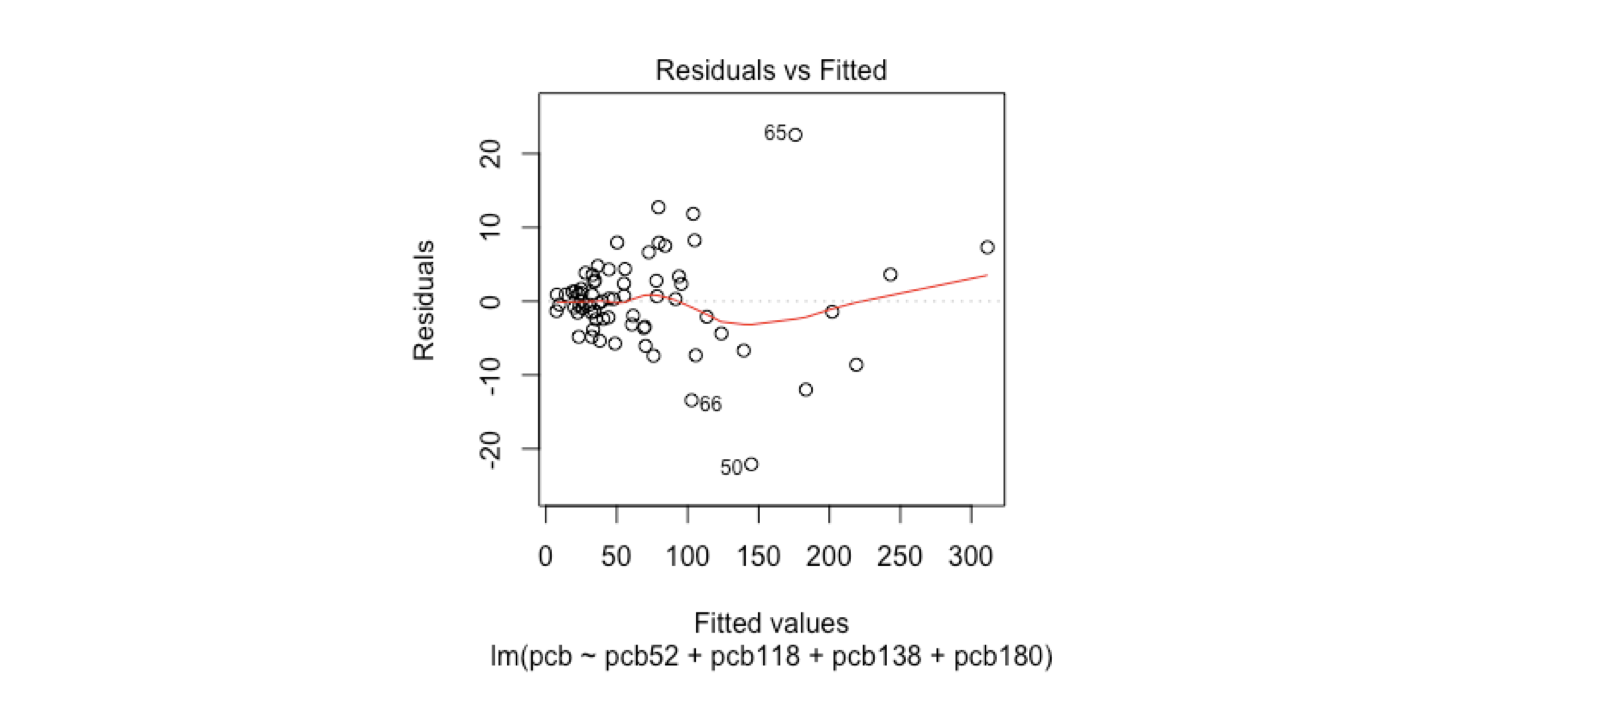
\includegraphics[width=.9\linewidth]{./graphs/image6.png}
\end{center}
The specimen 50 and 65 are the two data points that are outliers. Specimen 65 corresponds to an overestimate of PCB due to its higher residual value. 

\subsubsection*{(b) Rerun the analysis with the two suspected outliers deleted, summarize these results, and compare them with those you obtained in the previous exercise.}
\label{sec:orgb283455}

\begin{verbatim}
(Intercept)       pcb52      pcb118      pcb138      pcb180 
   1.627718   14.442021    2.599636    4.054061    4.108575 
> summary(lm2)
Call:
lm(formula = pcb ~ pcb52 + pcb118 + pcb138 + pcb180, data = subdf2)

Residuals:
     Min       1Q   Median       3Q      Max 
-12.2421  -2.1762  -0.1378   1.7036  14.2051 

Coefficients:
            Estimate Std. Error t value Pr(>|t|)    
(Intercept)   1.6277     0.8858   1.838   0.0709 .  
pcb52        14.4420     0.6960  20.751  < 2e-16 ***
pcb118        2.5996     0.5164   5.034 4.40e-06 ***
pcb138        4.0541     0.3752  10.805 6.89e-16 ***
pcb180        4.1086     0.3175  12.942  < 2e-16 ***
---
Signif. codes:  0 ‘***’ 0.001 ‘**’ 0.01 ‘*’ 0.05 ‘.’ 0.1 ‘ ’ 1

Residual standard error: 4.555 on 62 degrees of freedom
Multiple R-squared:  0.9941,	Adjusted R-squared:  0.9938 
F-statistic:  2629 on 4 and 62 DF,  p-value: < 2.2e-16

> anova(lm2)
Analysis of Variance Table
Response: pcb
          Df Sum Sq Mean Sq F value    Pr(>F)    
pcb52      1  84307   84307  4062.7 < 2.2e-16 ***
pcb118     1  68740   68740  3312.6 < 2.2e-16 ***
pcb138     1  61670   61670  2971.9 < 2.2e-16 ***
pcb180     1   3476    3476   167.5 < 2.2e-16 ***
Residuals 62   1287      21                      
---
Signif. codes:  0 ‘***’ 0.001 ‘**’ 0.01 ‘*’ 0.05 ‘.’ 0.1 ‘ ’ 1
\end{verbatim}
The residual standard error has been decreased without the suspected outliers, from 6.382 to 4.555. R\(^{\text{2}}\) has also increased from 0.989 to 0.994, meaning the predictions with this dataset become more accurate. 

\subsection*{11.45 More on predicting the total amount of PCB.}
\label{sec:org99ce0dd}
Run a regression to predict PCB using the variables PCB52, PCB118, and PCB138. Note that this is similar to the analysis that you did in Exercise 11.43, with the change that PCB 180 is not included as an explanatory variable. 
\subsubsection*{(a) Summarize the results.}
\label{sec:orgac7a70a}

\begin{verbatim}
> coef(lm3)
(Intercept)       pcb52      pcb118      pcb138 
 -1.0183987  12.6441934   0.3131051   8.2545867 
> summary(lm3)
Call:
lm(formula = pcb ~ pcb52 + pcb118 + pcb138, data = subdf3)

Residuals:
     Min       1Q   Median       3Q      Max 
-29.6219  -3.3502   0.8791   3.3785  29.5217 

Coefficients:
            Estimate Std. Error t value Pr(>|t|)    
(Intercept)  -1.0184     1.8895  -0.539    0.592    
pcb52        12.6442     1.1291  11.198   <2e-16 ***
pcb118        0.3131     0.8333   0.376    0.708    
pcb138        8.2546     0.3279  25.177   <2e-16 ***
---
Signif. codes:  0 ‘***’ 0.001 ‘**’ 0.01 ‘*’ 0.05 ‘.’ 0.1 ‘ ’ 1

Residual standard error: 9.945 on 65 degrees of freedom
Multiple R-squared:  0.9732,	Adjusted R-squared:  0.972 
F-statistic: 786.7 on 3 and 65 DF,  p-value: < 2.2e-16

> anova(lm3)
Analysis of Variance Table
Response: pcb
          Df Sum Sq Mean Sq F value    Pr(>F)    
pcb52      1  85302   85302  862.48 < 2.2e-16 ***
pcb118     1  85429   85429  863.77 < 2.2e-16 ***
pcb138     1  62693   62693  633.88 < 2.2e-16 ***
Residuals 65   6429      99                      
---
Signif. codes:  0 ‘***’ 0.001 ‘**’ 0.01 ‘*’ 0.05 ‘.’ 0.1 ‘ ’ 1
\end{verbatim}
We can get the following values from the results of the regression:
\begin{itemize}
\item The squared multiple correlation coeffiicient R\(^{\text{2}}\) = 0.973
\item The residual standard error SE = 9.942
\end{itemize}

\subsubsection*{(b) In this analysis, the regression coefficient for PCB118 is not statistically significant. Give the estimate of the coefficient and the associated \emph{P}-value.}
\label{sec:org7cc638e}

\begin{itemize}
\item Using a significance level \(\alpha\) = 0.05, Specimen PCB118 has a regression coefficient = 0.313 and \emph{P}-value = 0.708
\item Significance Test: 0.708 > 0.05 (Reject when P > \(\alpha\))
\item \emph{P}-value is much larger than the significance level. Therefore, we reject the null hypothesis.
\end{itemize}

\subsubsection*{(c) Find the estimate of the coefficient for PCB118 and the associated \emph{P}-value for the model analyzed the Ecercise 11.43.}
\label{sec:orgc77bbce}
\begin{itemize}
\item Using a significance level \(\alpha\) = 0.05, Specimen PCB118(from Exercise 11.43) has a regression coefficient = 3.7611 and \emph{P}-value = 0.000
\item Significance Test: 0.000 < 0.05 (Reject when P > \(\alpha\))
\item \emph{P}-value is much smaller than the significance level. Therefore, we don't reject the null hypothesis.
\end{itemize}

\subsubsection*{(d) Using the results in parts (b) and (c), write a short paragraph explaining how the inclusion of other variables in a multiple regression can have an effect on the estimate of a particular coefficient and the results of the associated significance test.}
\label{sec:orge877165}
As parts (b) and (c) of this exercise show, the statistical significance of another variable is changed entirely, just by removing one explanatory variable. In the case above, removing the explanatory variable PCB180 made another explanatory variable PCB118 no longer statistically significant, along with drastically changing the variables corresponding regression coefficient and P-value. 

\subsection*{11.46 Multiple regression model for total TEQ}
\label{sec:orgd74f8a3}
\subsubsection*{(a) Consider using a multiple regression to predict TEQ using the tree components TEQPCB, TEQDIOXIN, and TEQFURAN as explanatory variables. Write the multiple regression model in the form: TEQ = \(\beta_{\text{0}}\) + \(\beta_{\text{1}}\)TEQPCB + \(\beta_{\text{2}}\)TEQDIOXIN + \(\beta_{\text{3}}\)TEQFURAN + \(\epsilon\). Give numerical values for the parameters \(\beta_{\text{0}}\), \(\beta_{\text{1}}\), \(\beta_{\text{2}}\), and \(\beta_{\text{3}}\).}
\label{sec:orge51d712}

\(\beta_{\text{0}}\) = 0, \(\beta_{\text{1}}\) = 1, \(\beta_{\text{2}}\) = 1, \(\beta_{\text{3}}\) = 1

TEQ = 0 + 1 * TEQPCB + 1 * TEQDIOXIN + 1 * TEQFURAN

\subsubsection*{(b) The multiple regression model assumes that the \(\epsilon\)'s are Normal with mean zero and standard deviation \(\sigma\). What is the numerical value of \(\sigma\)?}
\label{sec:orgc4bff81}
\(\sigma\) = s = 7.95e-6
\subsubsection*{(c) Use software to run this regression and summarize the results.}
\label{sec:org442bc43}

\begin{verbatim}
> lm4 <- lm(teq~teqpcb+teqdioxin+teqfuran, data=df)
> coef(lm4)
 (Intercept)       teqpcb    teqdioxin     teqfuran 
3.425522e-07 1.000001e+00 1.000000e+00 1.000001e+00 
> summary(lm4)

Call:
lm(formula = teq ~ teqpcb + teqdioxin + teqfuran, data = df)

Residuals:
       Min         1Q     Median         3Q        Max 
-5.638e-06 -2.844e-06 -1.680e-06 -1.130e-06  3.714e-05 

Coefficients:
             Estimate Std. Error   t value Pr(>|t|)    
(Intercept) 3.426e-07  1.917e-06 1.790e-01    0.859    
teqpcb      1.000e+00  8.239e-07 1.214e+06   <2e-16 ***
teqdioxin   1.000e+00  1.761e-06 5.677e+05   <2e-16 ***
teqfuran    1.000e+00  5.664e-06 1.766e+05   <2e-16 ***
---
Signif. codes:  0 ‘***’ 0.001 ‘**’ 0.01 ‘*’ 0.05 ‘.’ 0.1 ‘ ’ 1

Residual standard error: 7.95e-06 on 65 degrees of freedom
Multiple R-squared:      1,	Adjusted R-squared:      1 
F-statistic: 9.581e+11 on 3 and 65 DF,  p-value: < 2.2e-16

> anova(lm4)
Analysis of Variance Table
Response: teq
          Df  Sum Sq Mean Sq    F value    Pr(>F)    
teqpcb     1 152.801 152.801 2.4174e+12 < 2.2e-16 ***
teqdioxin  1  26.903  26.903 4.2562e+11 < 2.2e-16 ***
teqfuran   1   1.970   1.970 3.1174e+10 < 2.2e-16 ***
Residuals 65   0.000   0.000                         
---
Signif. codes:  0 ‘***’ 0.001 ‘**’ 0.01 ‘*’ 0.05 ‘.’ 0.1 ‘ ’ 1
\end{verbatim}
\begin{itemize}
\item We gathered the following values from the results of the regression:
\label{sec:org0765d2f}
\begin{itemize}
\item Multiple R-squared R\(^{\text{2}}\) = 1
\item Residual standard error SE = 7.95e-06 \(\approx\) 0
\end{itemize}
\end{itemize}

\item Test 1
\label{sec:org0609916}

H\(_{\text{0}}\) : \(\beta_{\text{0}}\) = \(\beta_{\text{1}}\) = \(\beta_{\text{2}}\) = \(\beta_{\text{3}}\) = \(\beta_{\text{4}}\) = 0

H\(_{\text{1}}\) : \(\beta_{\text{0}}\) \(\neq\) 0 \(\vee\) \(\beta_{\text{1}}\) \(\neq\) 0 \(\vee\) \(\beta_{\text{2}}\) \(\neq\) 0 \(\vee\) \(\beta_{\text{3}}\) \(\neq\) 0 \(\vee\) \(\beta_{\text{4}}\) \(\neq\) 0

Since there is at least one \(\beta_{\text{n}}\) \(\neq\) 0, we reject H\(_{\text{0}}\)

\item Test 2
\label{sec:org5ac48c8}

H\(_{\text{0}}\) = \(\beta_{\text{j}}\) = 0, \emph{j = 0, 1, 2, 3}

H\(_{\text{1}}\) = \(\beta_{\text{j}}\) \(\neq\) 0

All regression coefficients are significantly different from 0 with the exception of the constant R\(^{\text{1}}\) = 1, meaning 100\% of TEQ is explained by TEQPCB, TEQDIOXIN and TEQFURAN.
\end{itemize}

\subsection*{11.47 Multiple regression model for total TEQ, cont.}
\label{sec:org3e03355}
\begin{verbatim}
Call:
lm(formula = teq ~ pcb52 + pcb118 + pcb138 + pcb180, data = df)

Residuals:
    Min      1Q  Median      3Q     Max 
-1.6655 -0.6000 -0.1814  0.5162  2.7025 

Coefficients:
             Estimate Std. Error t value Pr(>|t|)    
(Intercept)  1.059965   0.184450   5.747 2.73e-07 ***
pcb52       -0.097277   0.109383  -0.889  0.37716    
pcb118       0.306184   0.096388   3.177  0.00229 ** 
pcb138       0.105786   0.074697   1.416  0.16156    
pcb180      -0.003905   0.064784  -0.060  0.95212    
---
Signif. codes:  0 ‘***’ 0.001 ‘**’ 0.01 ‘*’ 0.05 ‘.’ 0.1 ‘ ’ 1

Residual standard error: 0.9576 on 64 degrees of freedom
Multiple R-squared:  0.6769,	Adjusted R-squared:  0.6568 
F-statistic: 33.53 on 4 and 64 DF,  p-value: 4.489e-15

> summary(aov(lm5))
            Df Sum Sq Mean Sq F value   Pr(>F)    
pcb52        1  29.85   29.85  32.553 3.21e-07 ***
pcb118       1  83.61   83.61  91.174 6.30e-14 ***
pcb138       1   9.52    9.52  10.378  0.00201 ** 
pcb180       1   0.00    0.00   0.004  0.95212    
Residuals   64  58.69    0.92                     
---
Signif. codes:  0 ‘***’ 0.001 ‘**’ 0.01 ‘*’ 0.05 ‘.’ 0.1 ‘ ’ 1
\end{verbatim}
\subsubsection*{The regression equation used:}
\label{sec:org1310cbb}
TEQ = 1.06 − 0.097 ∗ PCB52 + 0.306 ∗ PCB118 + 0.106 ∗ PCB138 − 0.0039 ∗ PCB180
\begin{itemize}
\item Multiple R-squared R\(^{\text{2}}\) = 0.6772
\item Residual standard error SE = 0.9571
\end{itemize}

\subsubsection*{Significance Test:}
\label{sec:org0995582}
\begin{itemize}
\item H\(_{\text{0}}\) = \(\beta_{\text{1}}\) = \(\beta_{\text{2}}\) = \(\beta_{\text{3}}\) = \(\beta_{\text{4}}\) = 0
\item H\(_{\text{a}}\) : one or more \(\beta\) \(\neq\) 0
\item The \emph{P}-value of both PCB118 and constant are close to 0, but still significantly different, therefore we reject null hypothesis.
\end{itemize}

\begin{center}
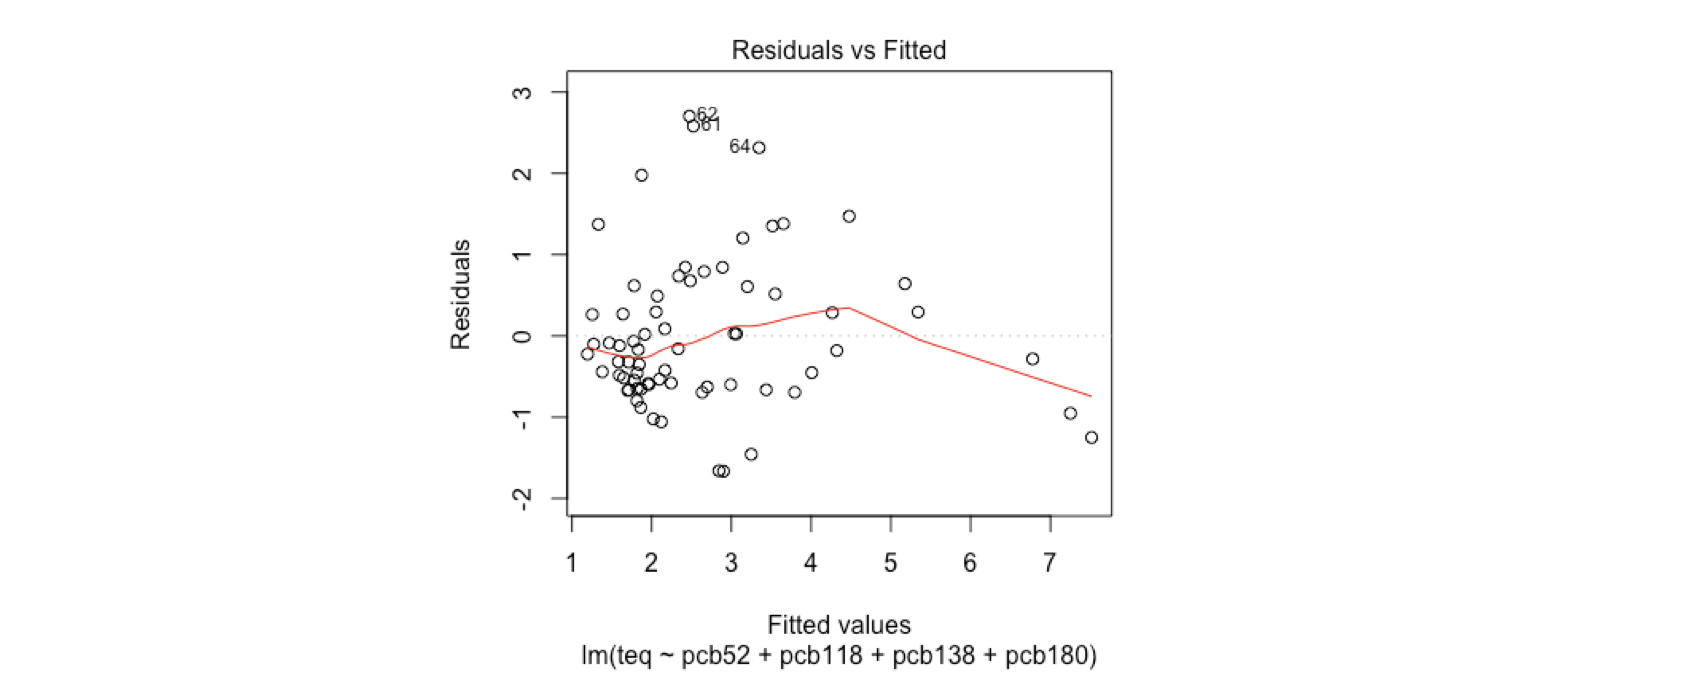
\includegraphics[width=.9\linewidth]{./graphs/image7.png}
\end{center}
When plotting the residuals, the data is skewed right but does not include any other obvious patterns. 

\subsection*{11.48 Predicting total amount of PCB using transformed variables}
\label{sec:org5390d6e}
Because distributions of variables such as PCB, the PCB congeners, and TEQ tend to be skewed, researchers frequently analyze the logarithms of the measured variables. Create a data set that has the logs of each of the variables in the PCB data file. Note that zero is a possible value for PCB126; most software packages will eliminate these cases when you request a log transformation.

\subsubsection*{(a) If you do not do anything about the 16 zero values of PCB126, what does your software do with these cases? Is there an error message of some kind?}
\label{sec:org1144f9d}
In the case of using the R language, the software will replace all the zero values with '-inf' without error.

\subsubsection*{(b) If you attempt to run a regression to predict the log of PCB using the log of PCB126 and the log of PCB52, are the cases with the zero values of PCB126 eliminated? Do you think that this is a good way to handle this situation?}
\label{sec:org2e6aa97}
In the case of the R language, the zero cases will remain and there will be no errors reported and it will perform the calculation, which can be beneficial. If there are zero's that are not intended, however, the software will not inform you. 

\subsubsection*{(c) The smallest nonzero value of PCB126 is 0.0052. One common practice when taking logarithms of measured values is to replace the zeros by one-half of the smallest observed value. Create a logarithm data set using this procedure; that is, replace the 16 zero values of PCB126 by 0.0026 before taking logarithms. Use numerical and graphical summaries to describe the distribution of the log variables.}
\label{sec:orgb891314}
\begin{verbatim}
    pcb138            pcb153            pcb180            pcb28             pcb52        
Min.   :-0.4463   Min.   :-0.1508   Min.   :-0.9289   Min.   :-5.1160   Min.   :-3.9120  
1st Qu.: 1.1569   1st Qu.: 1.1939   1st Qu.: 0.2151   1st Qu.:-2.0715   1st Qu.:-1.4784  
Median : 1.5933   Median : 1.6938   Median : 0.9895   Median :-1.3394   Median :-0.7402  
Mean   : 1.6139   Mean   : 1.7033   Mean   : 0.9752   Mean   :-1.3338   Mean   :-0.7722  
3rd Qu.: 2.1576   3rd Qu.: 2.2895   3rd Qu.: 1.5019   3rd Qu.:-0.8393   3rd Qu.:-0.1143  
Max.   : 3.4751   Max.   : 3.7728   Max.   : 3.4500   Max.   : 1.9359   Max.   : 2.2039  
    pcb126           pcb118             pcb             teq               teqpcb        
Min.   :-5.952   Min.   :-1.4439   Min.   :1.808   Min.   :-0.06358   Min.   :-2.68282  
1st Qu.:-5.221   1st Qu.: 0.3988   1st Qu.:3.407   1st Qu.: 0.30565   1st Qu.:-0.07958  
Median :-4.906   Median : 0.8838   Median :3.870   Median : 0.72609   Median : 0.23373  
Mean   :-4.846   Mean   : 0.8559   Mean   :3.917   Mean   : 0.80475   Mean   : 0.15422  
3rd Qu.:-4.220   3rd Qu.: 1.3584   3rd Qu.:4.518   3rd Qu.: 1.31648   3rd Qu.: 0.87228  
Max.   :-3.451   Max.   : 2.9392   Max.   :5.764   Max.   : 1.87074   Max.   : 1.68953  
  teqdioxin            teqfuran      
Min.   :-5.952244   Min.   :-5.9522  
1st Qu.:-1.505078   1st Qu.:-2.1804  
Median :-0.440787   Median :-1.6623  
Mean   :-0.853919   Mean   :-1.7870  
3rd Qu.: 0.004988   3rd Qu.:-1.2090  
Max.   : 1.178150   Max.   : 0.1187  
\end{verbatim}

\begin{center}
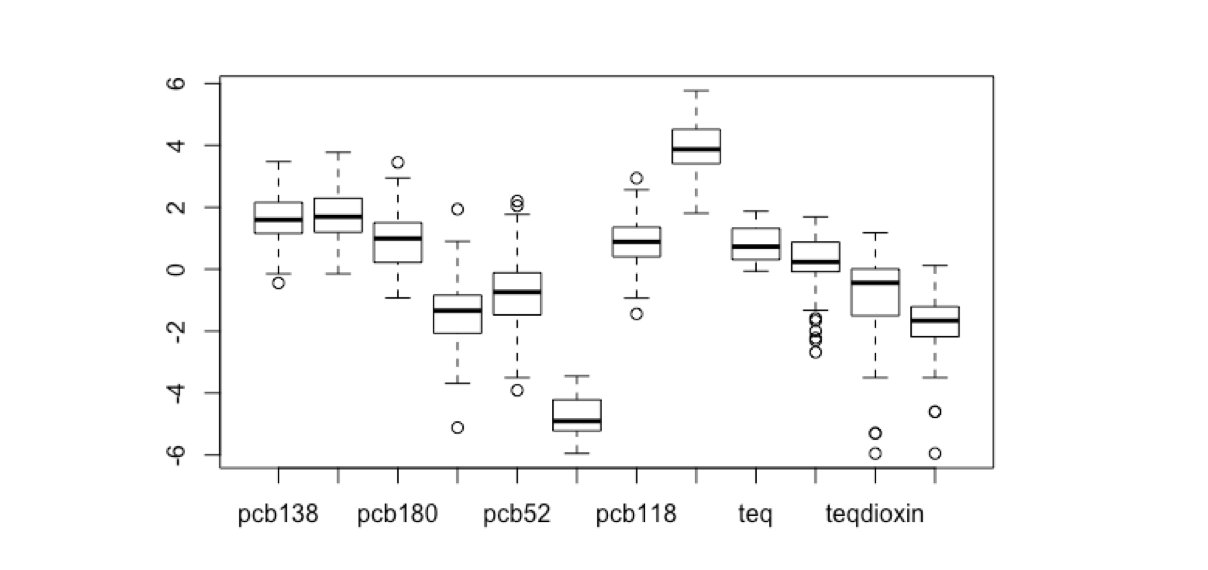
\includegraphics[width=.9\linewidth]{./graphs/image8.png}
\end{center}
From the plots, we can conclude that the data is approximately normal. 

\subsection*{11.49 Prediction total amount of PCB using transformed variables, continued.}
\label{sec:org99c3816}
\subsubsection*{(a) Use numerical and graphical summaries to describe the relationships between each pair of log variables}
\label{sec:orga336b0c}
\begin{center}
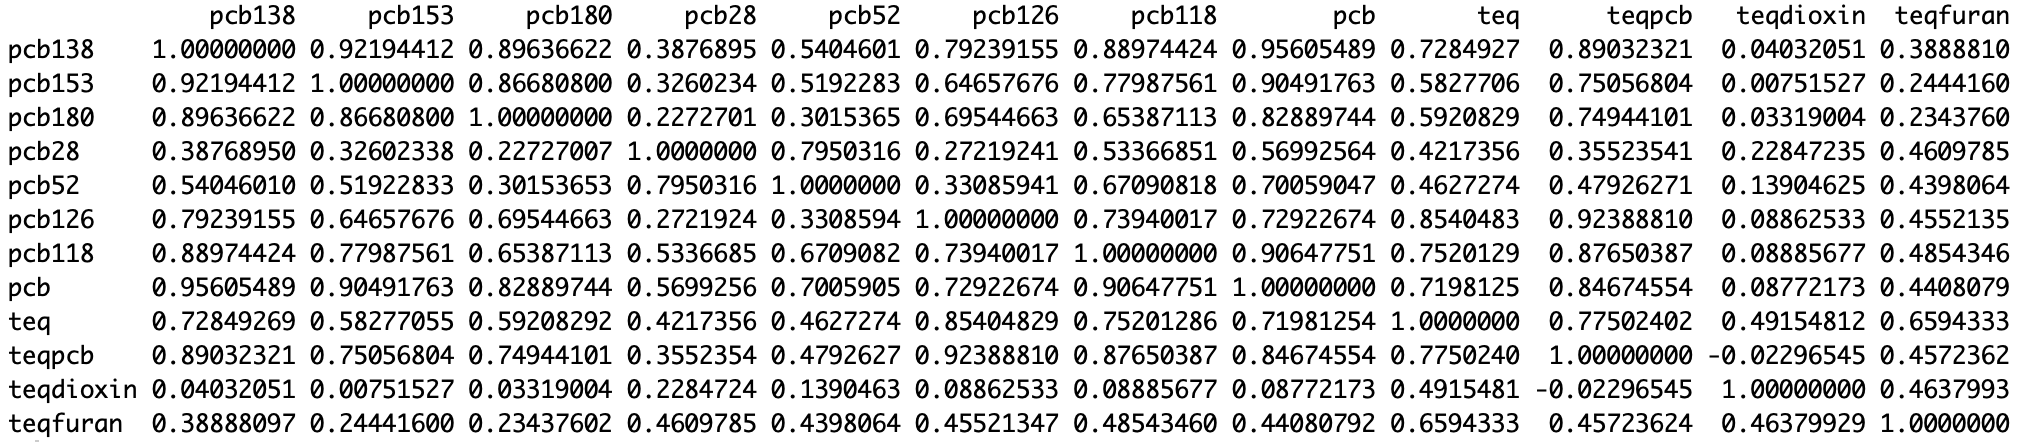
\includegraphics[width=.9\linewidth]{./graphs/image10.png}
\end{center}
\begin{center}
\includegraphics[width=.9\linewidth]{./graphs/image9.png}
\end{center}
All of the pairs shown in the above correlation table have a positive value for their correlation. There is one outlier in the pcb28, otherwise all charts are linearly correlated. 
\subsubsection*{(b) Compare these summaries with the summaries that you produced in Exercise 11.42 for the measured variables.}
\label{sec:org88a5566}
All pairs are positively correlated. As the log values get higher the correlations appear to be higher. 

\subsection*{11.50 Even more on predicting total amount of PCB using transformed variables.}
\label{sec:org1e51d79}
Use the log data set that you created in Exercise 11.48 to find a good multiple regression model for predicting the log of PCB. Use only log PCB variables for this analysis. Write a report summarizing your results.

\begin{verbatim}
Call:
lm(formula = pcb ~ (pcb52 + pcb118 + pcb138 + pcb153 + pcb180 + 
    pcb28 + pcb126), data = df_log)

Residuals:
     Min       1Q   Median       3Q      Max 
-0.28190 -0.07000 -0.01204  0.04450  0.51501 

Coefficients:
            Estimate Std. Error t value Pr(>|t|)    
(Intercept) 2.986842   0.253510  11.782  < 2e-16 ***
pcb52       0.101588   0.029763   3.413  0.00115 ** 
pcb118      0.150074   0.066788   2.247  0.02827 *  
pcb138      0.395901   0.127410   3.107  0.00287 ** 
pcb153      0.146018   0.053529   2.728  0.00831 ** 
pcb180      0.132351   0.061925   2.137  0.03659 *  
pcb28       0.087940   0.025828   3.405  0.00118 ** 
pcb126      0.003972   0.038703   0.103  0.91858    
---
Signif. codes:  0 ‘***’ 0.001 ‘**’ 0.01 ‘*’ 0.05 ‘.’ 0.1 ‘ ’ 1

Residual standard error: 0.135 on 61 degrees of freedom
Multiple R-squared:  0.9746,	Adjusted R-squared:  0.9717 
F-statistic: 334.2 on 7 and 61 DF,  p-value: < 2.2e-16

> anova(lm6)
Analysis of Variance Table

Response: pcb
          Df  Sum Sq Mean Sq   F value    Pr(>F)    
pcb52      1 21.4665 21.4665 1178.3204 < 2.2e-16 ***
pcb118     1 15.1504 15.1504  831.6213 < 2.2e-16 ***
pcb138     1  5.4596  5.4596  299.6863 < 2.2e-16 ***
pcb153     1  0.1279  0.1279    7.0217  0.010242 *  
pcb180     1  0.2074  0.2074   11.3855  0.001291 ** 
pcb28      1  0.2120  0.2120   11.6380  0.001152 ** 
pcb126     1  0.0002  0.0002    0.0105  0.918584    
Residuals 61  1.1113  0.0182                        
---
Signif. codes:  0 ‘***’ 0.001 ‘**’ 0.01 ‘*’ 0.05 ‘.’ 0.1 ‘ ’ 1
\end{verbatim}
The results of this mode: 
\begin{itemize}
\item Multiple R\(^{\text{2}}\) = 0.9751
\item Residual standard error SE = 0.135
\end{itemize}

The correlation coefficients for the data are also all positive. To say we have found the best fit, all assumptions made under the least squares regression should be upheld

\begin{center}
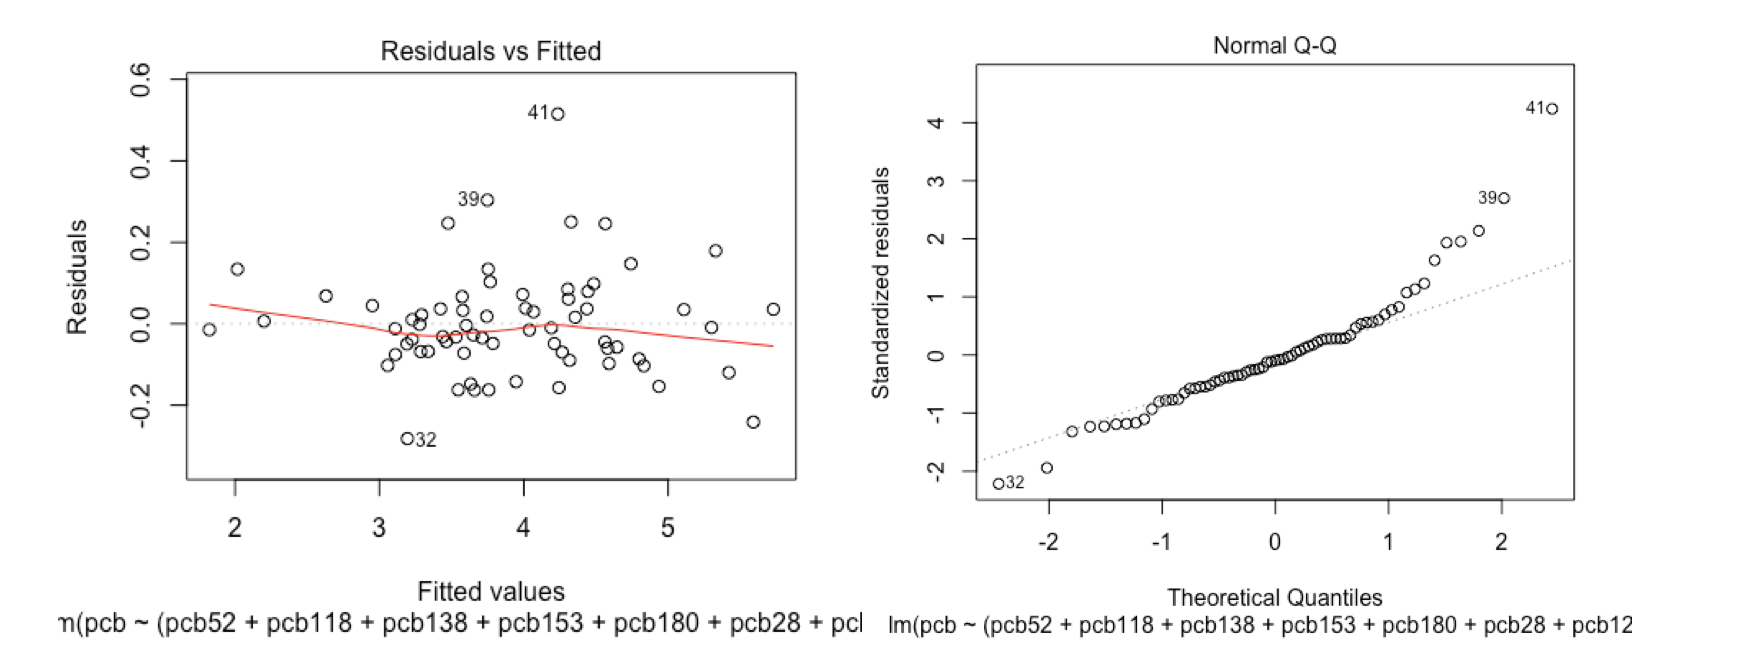
\includegraphics[width=.9\linewidth]{./graphs/image11.png}
\end{center}

Since these plots show approximately normal residuals, roughly linear relationships, independence and the assumptions are said to be upheld and the model is said to be a good fit. 

\subsection*{11.51 Predicting total TEQ using transformed variables.}
\label{sec:org10f4715}
Use the log data set that you created in Exercise 11.48 to find a good multiple regression model for predicting the log of TEQ. Use only log PCB variables for this analysis. Write a report summarizing your results and comparing them with the results that you obtained in the previous exercise. 

\begin{verbatim}
Call:
lm(formula = teq ~ (pcb52 + pcb118 + pcb138 + pcb153 + pcb180 + 
    pcb28 + pcb126), data = df_log)

Residuals:
     Min       1Q   Median       3Q      Max 
-0.53673 -0.18249  0.00731  0.14905  1.00180 

Coefficients:
            Estimate Std. Error t value Pr(>|t|)    
(Intercept)  3.69833    0.55220   6.697 7.65e-09 ***
pcb52        0.04209    0.06483   0.649    0.519    
pcb118       0.19173    0.14548   1.318    0.192    
pcb138      -0.08939    0.27753  -0.322    0.748    
pcb153      -0.09030    0.11660  -0.774    0.442    
pcb180       0.06266    0.13489   0.465    0.644    
pcb28        0.04508    0.05626   0.801    0.426    
pcb126       0.56299    0.08430   6.678 8.25e-09 ***
---
Signif. codes:  0 ‘***’ 0.001 ‘**’ 0.01 ‘*’ 0.05 ‘.’ 0.1 ‘ ’ 1

Residual standard error: 0.294 on 61 degrees of freedom
Multiple R-squared:  0.7822,	Adjusted R-squared:  0.7572 
F-statistic: 31.29 on 7 and 61 DF,  p-value: < 2.2e-16

> anova(lm7)
Analysis of Variance Table

Response: teq
          Df Sum Sq Mean Sq F value    Pr(>F)    
pcb52      1 5.1828  5.1828 59.9597 1.217e-10 ***
pcb118     1 8.5829  8.5829 99.2955 2.041e-14 ***
pcb138     1 0.3628  0.3628  4.1973  0.044797 *  
pcb153     1 0.7742  0.7742  8.9565  0.003987 ** 
pcb180     1 0.0777  0.0777  0.8988  0.346847    
pcb28      1 0.0974  0.0974  1.1267  0.292670    
pcb126     1 3.8550  3.8550 44.5985 8.254e-09 ***
Residuals 61 5.2727  0.0864                      
---
Signif. codes:  0 ‘***’ 0.001 ‘**’ 0.01 ‘*’ 0.05 ‘.’ 0.1 ‘ ’ 1
\end{verbatim}



\subsection*{11.52 Interpretation of coefficients in log PCB regressions}
\label{sec:org99acc2a}
Use the results of your analysis of the log PCB data in Exercise 11.50 to write an explanation of how regression coefficients, standard errors of regression coefficients, and tests of significance for explanatory variables can change depending on what other explanatory variables are included in the multiple regression analysis 
\end{document}
